\documentclass[12pt]{article}

\setlength{\topmargin}{-.75in} \addtolength{\textheight}{2.00in}
\setlength{\oddsidemargin}{.00in} \addtolength{\textwidth}{.75in}

\usepackage{amsmath,color,graphicx,array,multirow,rotating, enumerate}
\usepackage{type1cm}
\usepackage{eso-pic}
\usepackage[hmargin=2cm,vmargin=1.3cm]{geometry}
\usepackage{mathabx}
\usepackage[rflt]{/Users/jgates/desktop/latex/floatflt}
\usepackage[table]{xcolor}
\nofiles

\def\Tab#1{\tabular[t]{>{\rule[-1ex]{0pt}{3ex}}c}#1\endtabular}
\newcolumntype{C}{@{}c@{}}

\pagestyle{empty}
\newcounter{ProbNum}
\setlength{\parindent}{0in}

% Watermark: graph paper
\newcommand\BackgroundPic{
\put(0,0){
\parbox[b][\paperheight]{\paperwidth}{%
\vfill
\centering

\includegraphics[width=\paperwidth,height=\paperheight,keepaspectratio]{/Users/jgates/desktop/latex/pics/plain.pdf}%
\vfill
}}}

%Diagram box command [v space][content]
\newcommand{\diagrambox}[2][40 mm]{
\framebox{\parbox{175 mm}{#2 \hfill \\ \vspace{#1}}}

\bigskip
}

% MakeList: [example number] [content]
\newcommand{\MakeList}[2]{
\begin{enumerate}[#1] \itemsep1pt \parskip0pt \parsep0pt  

#2
\end{enumerate}
}

\begin{document}



{\Large Problems tagged with standards:}CVPMA
\bigskip 
% Number 130
% CVPMA Algebra Units
% Raptor/BSG drifting apart
% JG

% Watermark
\AddToShipoutPicture*{\BackgroundPic}

\addtocounter {ProbNum} {1}

%\begin{floatingfigure}[r]{.3\textwidth}
%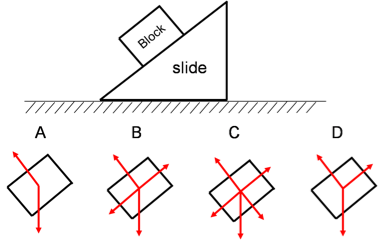
\includegraphics[scale=.4]{/Users/jgates/desktop/latex/pics/incline3.png}
%\end{floatingfigure}
 
{\bf \Large{130.}} Gaeta's Raptor is drifting away from Galactica at a speed of 200 meters per second, while the Galactica drifts away from the Raptor at a speed of 75 meters per second.  The two ships are initially 300 km away from each other.

\bigskip

\indent  How much time will pass before they are 600 km away from each other, and communication is lost?

\bigskip 
\vspace{6mm}% Number 160
% CVPMA Units Algebra Prefixes
% Problem-solving, Nostromo signal - hard!
% JG

% Watermark
\AddToShipoutPicture*{\BackgroundPic}

\addtocounter {ProbNum} {1}

%\begin{floatingfigure}[r]{.3\textwidth}
%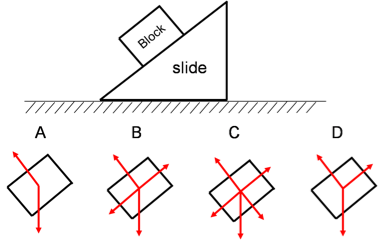
\includegraphics[scale=.4]{/Users/jgates/desktop/latex/pics/incline3.png}
%\end{floatingfigure}
 
{\bf \Large{160.}} As its crew sleeps, the Nostromo glides through space at a brisk clip of ${920~\tfrac{km}{s}}$, relative to a nearby asteroid that it is approaching.  The computer uses radar (object detection using radio waves, which travel at the speed of light: ${3 \times 10^8 ~\tfrac{m}{s}}$) to detect objects in the ship's path.  The radio waves are emitted by the ship, bounce off of the asteroid, and return to the ship, where the computer analyzes the results.

\bigskip
Assume that the asteroid begins at the limit of the ship's effective radar range of 2 million km.  Once it detects the asteroid, the computer will require 15 minutes to revive the crew.  

\bigskip

How much time will the crew have to turn the ship at that point?
%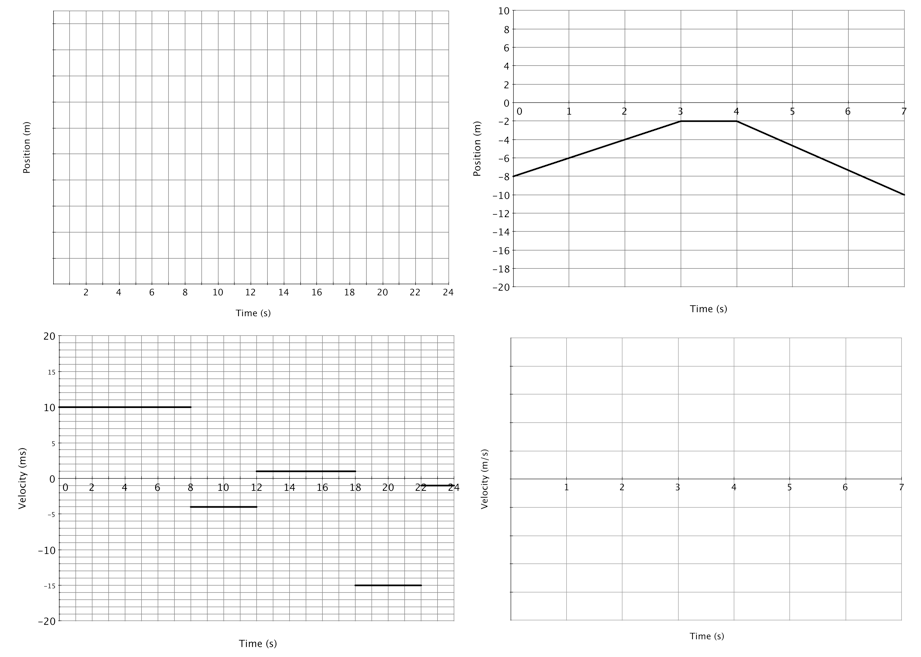
\includegraphics[scale=.57]{/Users/jgates/desktop/latex/pics/cvpmgraphs1.png}

\bigskip 
\vspace{6mm}% Number 160
% CVPMA Algebra Units Prefixes
% Problem-solving, Nostromo signal - hard!
% JG

% Watermark
\AddToShipoutPicture*{\BackgroundPic}

\addtocounter {ProbNum} {1}

%\begin{floatingfigure}[r]{.3\textwidth}
%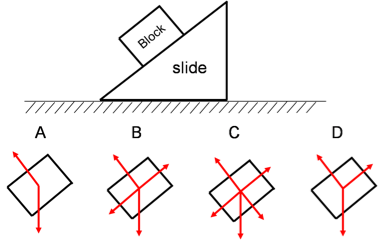
\includegraphics[scale=.4]{/Users/jgates/desktop/latex/pics/incline3.png}
%\end{floatingfigure}
 
{\bf \Large{170.}} As its crew sleeps, the Nostromo glides through space at a brisk clip of ${920~\tfrac{km}{s}}$, relative to a nearby asteroid that it is approaching.  The computer uses radar (object detection using radio waves, which travel at the speed of light: ${3 \times 10^8 ~\tfrac{m}{s}}$) to detect objects in the ship's path.  The radio waves are emitted by the ship, bounce off of the asteroid, and return to the ship, where the computer analyzes the results.

\bigskip
Assume that the asteroid begins at the limit of the ship's effective radar range of 2 million km.  Once it detects the asteroid, the computer will require 15 minutes to revive the crew.  

\bigskip

How much time will the crew have to turn the ship at that point?
%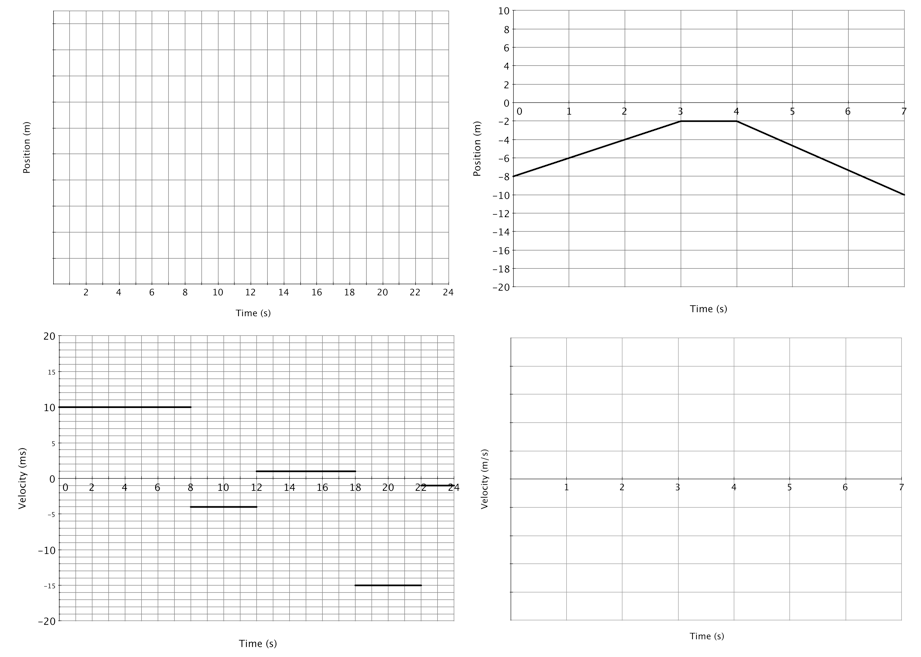
\includegraphics[scale=.57]{/Users/jgates/desktop/latex/pics/cvpmgraphs1.png}

\bigskip 
\vspace{6mm}% Number 180
% CVPMA Algebra Units 
% Problem-solving, RC cars passing each other - hardish
% JG

% Watermark
\AddToShipoutPicture*{\BackgroundPic}

\addtocounter {ProbNum} {1}

%\begin{floatingfigure}[r]{.3\textwidth}
%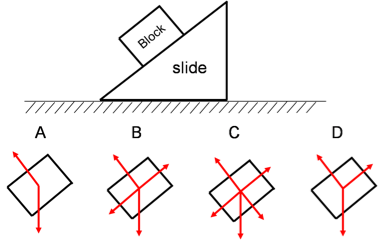
\includegraphics[scale=.4]{/Users/jgates/desktop/latex/pics/incline3.png}
%\end{floatingfigure}
 
{\bf \Large{180.}} A fast RC car (speed: ${12~\tfrac{m}{s}}$ and a slower RC car (${8~\tfrac{m}{s}}$) are 40 meters apart. They then drive directly towards each other.  Some time after the cars have passed each other, the faster car is 15 meters away from the slower one.  

\bigskip

At this moment, how far has the slower one traveled from its starting position? 

%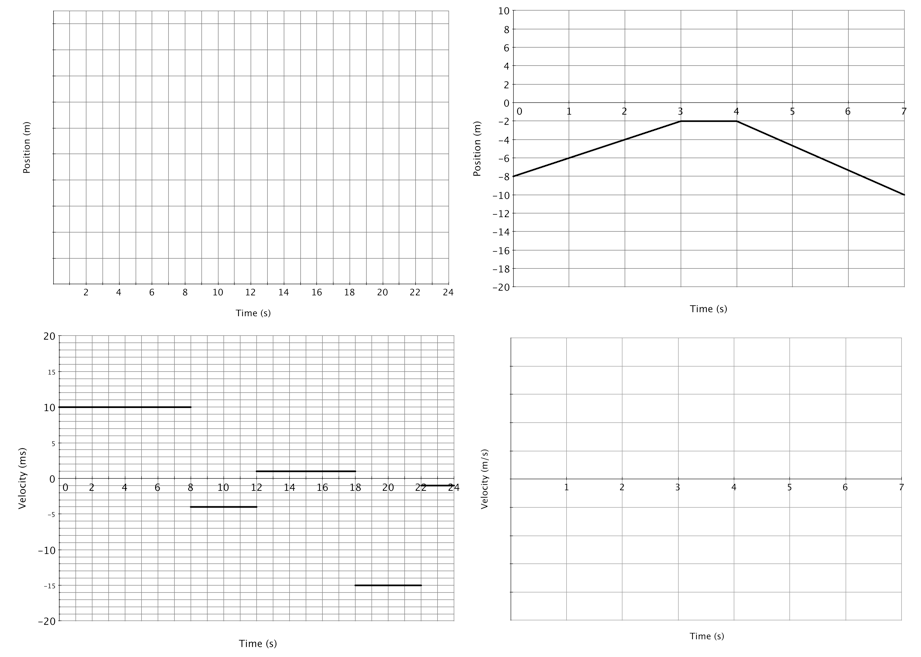
\includegraphics[scale=.57]{/Users/jgates/desktop/latex/pics/cvpmgraphs1.png}

\bigskip 
\vspace{6mm}% Number 190
% CVPMA Algebra Units OddUnits
% Problem-solving, mile marker problem
% Walker

% Watermark
\AddToShipoutPicture*{\BackgroundPic}

\addtocounter {ProbNum} {1}

%\begin{floatingfigure}[r]{.3\textwidth}
%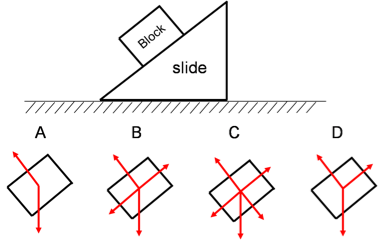
\includegraphics[scale=.4]{/Users/jgates/desktop/latex/pics/incline3.png}
%\end{floatingfigure}
 
{\bf \Large{190.}} You're driving along the highway at constant speed.  When you increase your speed by ${7.9~\tfrac{mi}{hr}}$, the time to go one mile decreases by 13 s. 

\bigskip

What was your original speed?  

%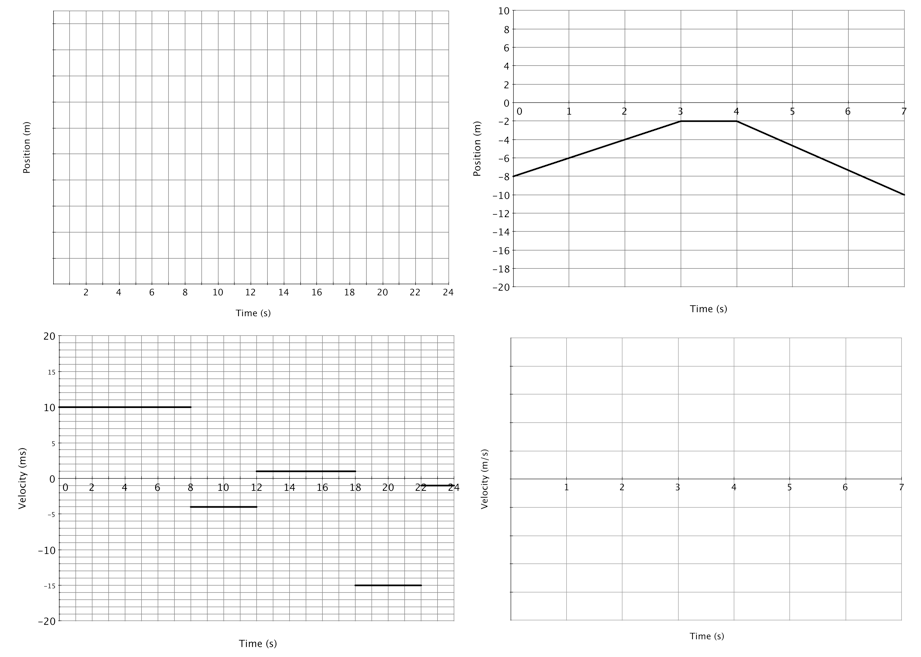
\includegraphics[scale=.57]{/Users/jgates/desktop/latex/pics/cvpmgraphs1.png}

\bigskip 
\vspace{6mm}% Number 210
% CVPMA Algebra Units
% Flipper: x modeling given graph
% JG

% Watermark
\AddToShipoutPicture*{\BackgroundPic}

\addtocounter {ProbNum} {1}

\begin{floatingfigure}[r]{.4\textwidth}
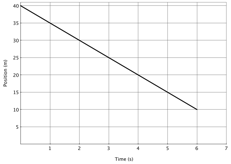
\includegraphics[scale=1]{/Users/jgates/desktop/latex/pics/flipper.png}
\end{floatingfigure}
 
{\bf \Large{210.}} Consider an x vs. t graph for Flipper (you know, the dolphin: king of the sea?).

\bigskip

Agebraically determine Flipper�s position at ${t =}$ 10 s.

%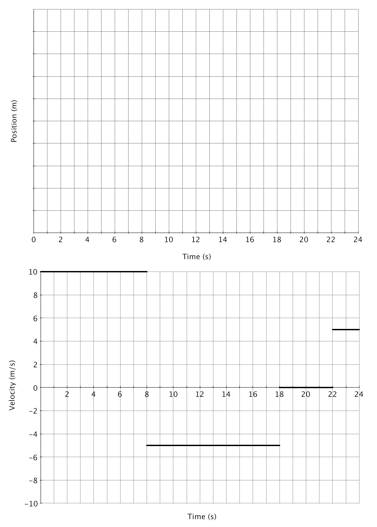
\includegraphics[scale=.77]{/Users/jgates/desktop/latex/pics/vtoxgraph1.png}

\bigskip 
\vspace{6mm}% Number 231
% CVPMA  Units
% Dori/Danica soccer: algebraic version
% JG

% Watermark
\AddToShipoutPicture*{\BackgroundPic}

\addtocounter {ProbNum} {1}

%\begin{floatingfigure}[r]{.4\textwidth}
%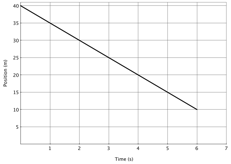
\includegraphics[scale=1]{/Users/jgates/desktop/latex/pics/flipper.png}
%\end{floatingfigure}
 
{\bf \Large{231.}} Dori's running at ${2~\tfrac{m}{s}}$ towards Tower Hill's goal line from 20 meters away when Danica lofts a ball over Dori's head.  The ball hits the ground 3 meters ahead of Dori and rolls towards the goal line at ${4~\tfrac{m}{s}}$.  

\bigskip

It takes 1.5 seconds for Dori to react to the ball; at that point, she begins running faster in order to catch up with the ball before it reaches the goal line.  
%\begin{center} 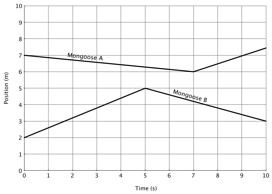
\includegraphics[scale=1]{/Users/jgates/desktop/latex/pics/mongooses.png}
%\end{center}

\bigskip

How fast does she need to run to catch up with the ball before it goes over the goal line? Use algebraic problem-solving.

\bigskip 
\vspace{6mm}% Number 240
% CVPMA Algebra  Units
% Football players running at each other: algebraic version
% JG

% Watermark
\AddToShipoutPicture*{\BackgroundPic}

\addtocounter {ProbNum} {1}

%\begin{floatingfigure}[r]{.4\textwidth}
%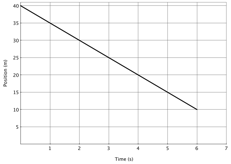
\includegraphics[scale=1]{/Users/jgates/desktop/latex/pics/flipper.png}
%\end{floatingfigure}
 
{\bf \Large{240.}} A running back carries the football down the field, running ${5.6~\tfrac{m}{s}}$.  The slower safety (running speed: ${4.5~\tfrac{m}{s}}$) runs towards him and tries to tackle him. They begin 22 meters apart and run straight at each other.  
%\begin{center} 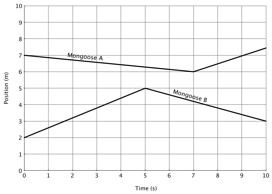
\includegraphics[scale=1]{/Users/jgates/desktop/latex/pics/mongooses.png}
%\end{center}

\bigskip

How far did the running back go before being tackled, and how much time elapsed before he was tackled? Draw a diagram and use algebraic problem solving.

 
\bigskip 
\vspace{6mm}% Number 250
% CVPMA Algebra Units
% Tron driving at each other
% JG

% Watermark
\AddToShipoutPicture*{\BackgroundPic}

\addtocounter {ProbNum} {1}

%\begin{floatingfigure}[r]{.3\textwidth}
%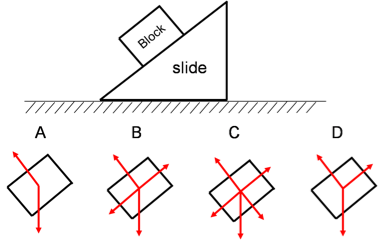
\includegraphics[scale=.4]{/Users/jgates/desktop/latex/pics/incline3.png}
%\end{floatingfigure}
 
{\bf \Large{250.}} Two lightcycles (like from Tron - that movie was awesome, and the remake wasn't bad) charge at each other from an initial distance of 112 meters.  One lightcyle has a constant speed of ${25~\tfrac{m}{s}}$, and the other a constant speed of ${32~\tfrac{m}{s}}$. They drive at each other, barely missing a head-on collision.  

%\begin{center}
%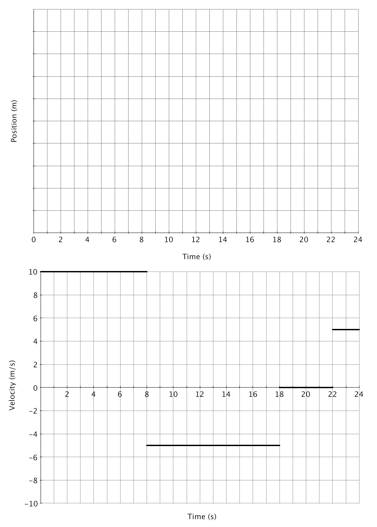
\includegraphics[scale=.77]{/Users/jgates/desktop/latex/pics/vtoxgraph1.png}
%\end{center}

\bigskip
Does CVPM apply? Why or why not?

\bigskip 
How long after they begin driving will they pass each other?
 
\bigskip 
\vspace{6mm}% Number 260
% CVPMA Algebra Units
% Model discrimination, avg v/speed
% JG

% Watermark
\AddToShipoutPicture*{\BackgroundPic}

\addtocounter {ProbNum} {1}

%\begin{floatingfigure}[r]{.3\textwidth}
%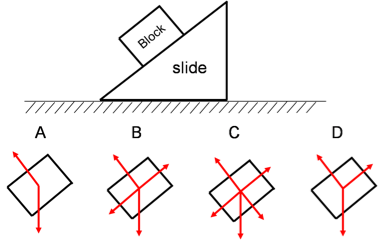
\includegraphics[scale=.4]{/Users/jgates/desktop/latex/pics/incline3.png}
%\end{floatingfigure}
 
{\bf \Large{260.}} A ball is thrown vertically into the air.  It takes 2.42 seconds for it to reach its peak height of 24.5 meters.

\bigskip
Does CVPM apply? Why or why not?

\bigskip 
\bigskip The ball will take another 2.42 seconds to hit the ground.  What is its average velocity over the whole trip?

\bigskip What was the ball's average speed during the whole trip?

%\begin{center}
%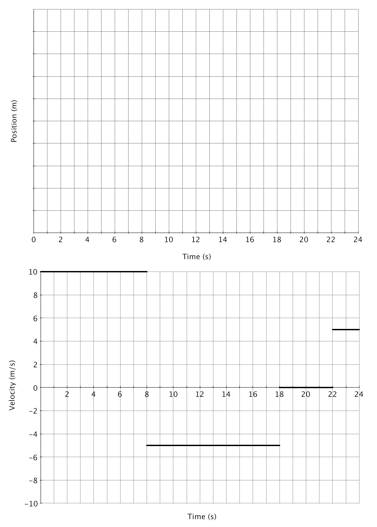
\includegraphics[scale=.77]{/Users/jgates/desktop/latex/pics/vtoxgraph1.png}
%\end{center}
 
\bigskip 
\vspace{6mm}% Number 270
% CVPMA Algebra Units
% Two objects moving, find collision time
% JG

% Watermark
\AddToShipoutPicture*{\BackgroundPic}

\addtocounter {ProbNum} {1}

%\begin{floatingfigure}[r]{.3\textwidth}
%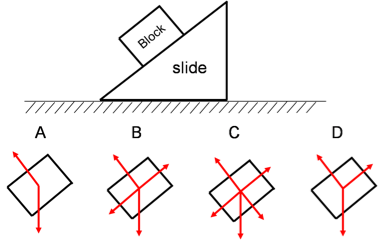
\includegraphics[scale=.4]{/Users/jgates/desktop/latex/pics/incline3.png}
%\end{floatingfigure}
 
{\bf \Large{270.}} Instead of waiting for a soccer pass to come to you, moving towards the ball can greatly increase your chances of not having the ball stolen.  A pass is made to you from 25 meters away, with a speed of ${13~\tfrac{m}{s}}$.  After a .4 second pause (your reaction time), you begin running towards the ball at ${5~\tfrac{m}{s}}$.

\bigskip
What issues might make a CVPM model of this situation less than faithful to the real situation?

\vspace{30mm}
Where (at what position) will you receive the pass?

%\begin{center}
%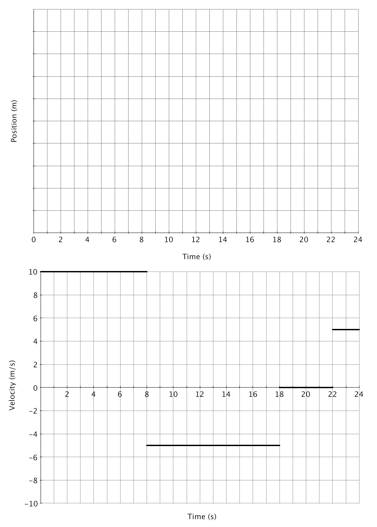
\includegraphics[scale=.77]{/Users/jgates/desktop/latex/pics/vtoxgraph1.png}
%\end{center}
 
\bigskip 
\vspace{6mm}% Number 280
% CVPMA Algebra Units
% Dune buggy overtaking, find distance
% JG

% Watermark
\AddToShipoutPicture*{\BackgroundPic}

\addtocounter {ProbNum} {1}

%\begin{floatingfigure}[r]{.3\textwidth}
%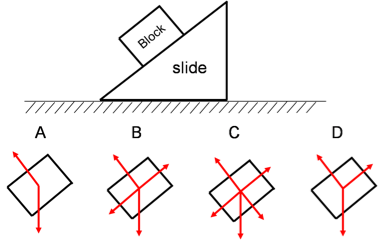
\includegraphics[scale=.4]{/Users/jgates/desktop/latex/pics/incline3.png}
%\end{floatingfigure}
 
{\bf \Large{280.}}A dune buggy takes off down the beach, driving ${8.9~\tfrac{m}{s}}$.  It then passes a second dune buggy, which sets off after it at a speed of ${12.1~\tfrac{m}{s}}$, after waiting four seconds to start.

\bigskip
Describe some ways in which a CVPM model of this situation would not match reality.

\bigskip How far has the first dune buggy traveled when it is caught by the second dune buggy?

%\begin{center}
%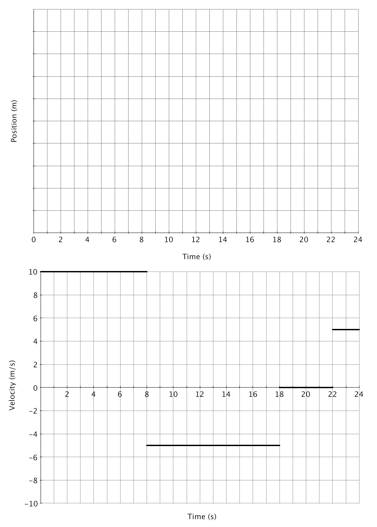
\includegraphics[scale=.77]{/Users/jgates/desktop/latex/pics/vtoxgraph1.png}
%\end{center}
 
\bigskip 
\vspace{6mm}% Number 281
% CVPMA Algebra Units
% Dune buggy overtaking, find time
% JG

% Watermark
\AddToShipoutPicture*{\BackgroundPic}

\addtocounter {ProbNum} {1}

%\begin{floatingfigure}[r]{.3\textwidth}
%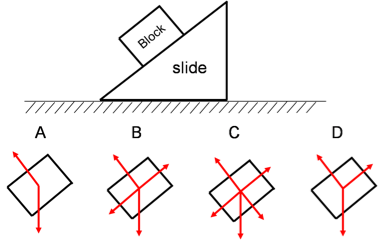
\includegraphics[scale=.4]{/Users/jgates/desktop/latex/pics/incline3.png}
%\end{floatingfigure}
 
{\bf \Large{281.}}A dune buggy takes off down the beach, driving ${8.9~\tfrac{m}{s}}$.  It then passes a second dune buggy, which sets off after it at a speed of ${12.1~\tfrac{m}{s}}$, after waiting four seconds to start.

\bigskip
Describe some ways in which a CVPM model of this situation would not match reality.

\bigskip For how long has the first dune buggy traveled when it is caught by the second dune buggy?

%\begin{center}
%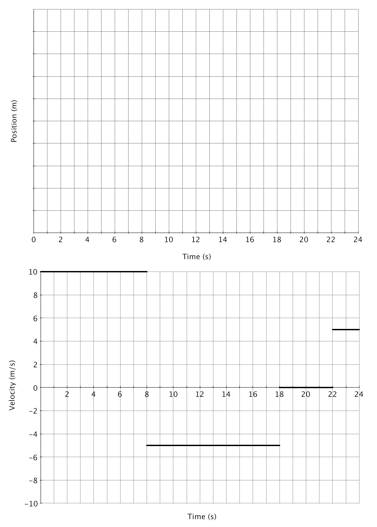
\includegraphics[scale=.77]{/Users/jgates/desktop/latex/pics/vtoxgraph1.png}
%\end{center}
 
\bigskip 
\vspace{6mm}% Number 290
% CVPMA Algebra Units
% Avg. v, speed, dsiplacement
% JG

% Watermark
\AddToShipoutPicture*{\BackgroundPic}

\addtocounter {ProbNum} {1}

%\begin{floatingfigure}[r]{.3\textwidth}
%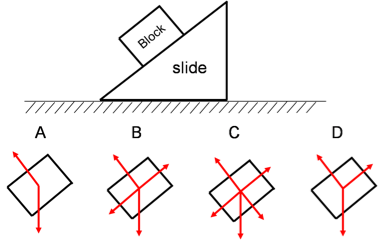
\includegraphics[scale=.4]{/Users/jgates/desktop/latex/pics/incline3.png}
%\end{floatingfigure}
 
{\bf \Large{290.}}A squirrel runs back and forth on a fence rail.  It runs east 4 meters in 1.2 seconds, then pauses for .8 seconds, then runs west 6 meters in 1.3 seconds, and then east 7 meters in 4 seconds.

\bigskip
What was the squirrel's maximum speed?

\bigskip 
\bigskip \bigskip What was the squirrel's displacement during the first 3 seconds?
 
%\begin{center}
%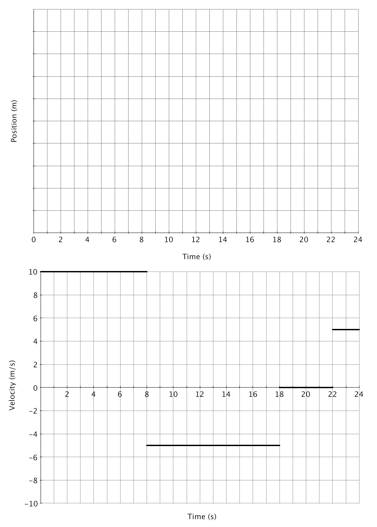
\includegraphics[scale=.77]{/Users/jgates/desktop/latex/pics/vtoxgraph1.png}
%\end{center}
 
\bigskip 
\vspace{6mm}% Number 321
% CVPMA Algebra Units
% Chase after distance pause: problem-solving
% JG

% Watermark
\AddToShipoutPicture*{\BackgroundPic}

\addtocounter {ProbNum} {1}

%\begin{floatingfigure}[r]{.3\textwidth}
%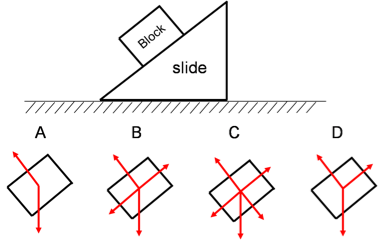
\includegraphics[scale=.4]{/Users/jgates/desktop/latex/pics/incline3.png}
%\end{floatingfigure}
 
{\bf \Large{321.}}A real police car chases down a stolen sturgeon truck.  The police car is sitting by the side of the road when the truck flies by at ${35~\tfrac{m}{s}}$.  Assume that the police officer reacts after the truck is 150 meters past her and gets up to speed instantly.  
 
%\begin{center}
%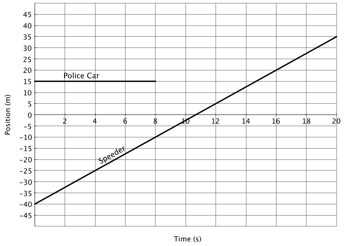
\includegraphics[scale=.87]{/Users/jgates/desktop/latex/pics/cvpm2.png}
%\end{center}

\bigskip
How fast does she need to go in order to catch the truck within 2 minutes? Use algebraic problem-solving.
 
\bigskip 
\vspace{6mm}% Number 325
% CVPMA Algebra Units
% Chase after time pause: problem-solving
% JG

% Watermark
\AddToShipoutPicture*{\BackgroundPic}

\addtocounter {ProbNum} {1}

%\begin{floatingfigure}[r]{.3\textwidth}
%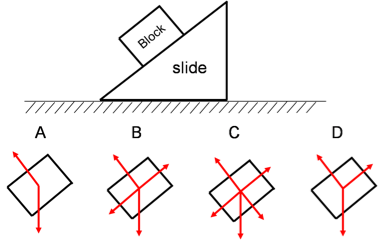
\includegraphics[scale=.4]{/Users/jgates/desktop/latex/pics/incline3.png}
%\end{floatingfigure}
 
{\bf \Large{325.}}A real police car chases down a stolen sturgeon truck.  The police car is sitting by the side of the road when the truck flies by at ${35~\tfrac{m}{s}}$.  The police officer takes 1.5 seconds to react, but we'll assume that she can get the car up to speed instantly.

%\begin{center}
%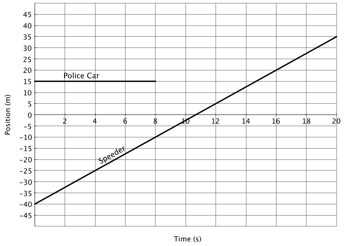
\includegraphics[scale=.87]{/Users/jgates/desktop/latex/pics/cvpm2.png}
%\end{center}

\bigskip
how fast will she have to go in order to catch the speeder within 2 km? Use algebraic problem-solving.
 
\bigskip 
\vspace{6mm}% Number 500
% CAPMA CVPMA 
% Stoplight stopping
% KO

% Watermark
\AddToShipoutPicture*{\BackgroundPic}

\addtocounter {ProbNum} {1}

%\begin{floatingfigure}[r]{.33\textwidth}
%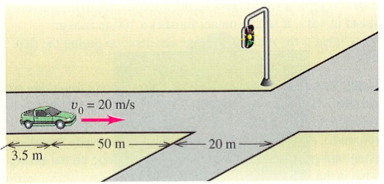
\includegraphics[scale=.6]{/Users/jgates/desktop/latex/pics/redlight}
%\end{floatingfigure}
 
{\bf \Large{500.}} A car 3.5 m in length and traveling at a constant speed of ${20~\tfrac{m}{s}}$ is approaching an intersection. The width of the intersection is 20 m. The light turns yellow when the front of the car is 50 m from the beginning of the intersection. If the driver steps on the brake, the car will slow at a rate of ${4.2~\tfrac{m}{s}}$ per second. If the driver instead steps on the gas pedal, the car will accelerate at ${1.5~\tfrac{m}{s^2}}$. The light will be yellow for 3 seconds. Ignore the reaction time of the driver. 

\bigskip
To avoid being in the intersection while the light is red, should the driver hit the brake pedal or the gas pedal? Justify your answer with some pretty physics.

\hfill 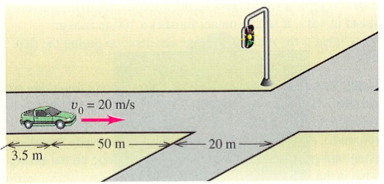
\includegraphics[scale=.85]{/Users/jgates/desktop/latex/pics/redlight.png}


\bigskip \vspace{6mm}% Number 540
% UFPM Vectors Algebra Units CAPMA CVPMA
% Wagon rolling down hill
% KO/JG

% Watermark
\AddToShipoutPicture*{\BackgroundPic}

\addtocounter {ProbNum} {1}

%\begin{floatingfigure}[r]{.45\textwidth}
%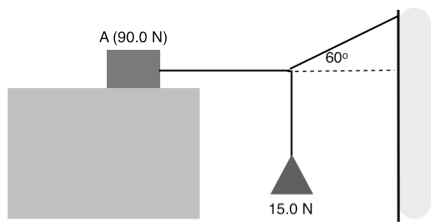
\includegraphics[scale=.6]{/Users/jgates/desktop/latex/pics/static1}
%\end{floatingfigure}
 
{\bf \Large{540.}} A wagon with two boxes of gold (total mass 300 kg) is cut loose from the horses by an outlaw when the wagon is at rest 50 m up a 6 degree slope. The outlaw plans to have the wagon roll down the slope and across the level ground, and then fall into a canyon where his confederates wait. 

\bigskip
Find the speed of the wagon when it reaches the flat ground. Note that it starts from rest at the top of the incline and that the wagon rolls with negligible friction.

\bigskip 
\bigskip If another bandit standing at the end of the slope requires twenty seconds to grab the gold, how far must the edge of the cliff be from the end of the slope, in order to make this double-heist successful?

%\hfill 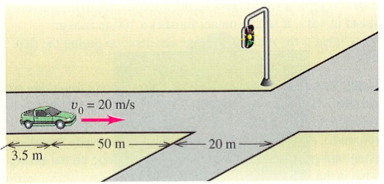
\includegraphics[scale=.85]{/Users/jgates/desktop/latex/pics/redlight.png}


\bigskip \vspace{6mm}\end{document}